% !TeX spellcheck = ru_RU
% !TEX root = vkr.tex

\section{Реализация}

В данном разделе представлены детали реализации алгоритма по генерации интерьера с учетом методов и технологий, рассмотренных в обзорной части. В частности, ниже представлены: подробное объяснения алгоритма PCG, архитектура библиотеки и тонкости ее интеграции с Unity проектом.

\subsection{Разделение комнаты на ячейки}

Перед процессом генерации помещение разделяется на клетки или \textit{ячейки}. Количество ячеек по вертикали и горизонтали в точности совпадает с измерениями комнаты: шириной и высотой. Ячейка определяет минимально возможную единицу комнаты для расстановки в ней мебели. Каждая ячейка имеет индекс по строке и столбцу на комнатной \textit{решетке}, а также текущее состояние или \textit{статус}. К ним относятся, например, \texttt{Occupied} и \texttt{NonOccupied}, обозначающие доступна ли рассматриваемая ячейка для размещения или нет. Стоит заметить, что координаты ячеек показывают расположение объектов на локальной сетке относительно друг друга и их показатели должны быть скорректированы для совпадения с координатной системой игры.

\subsection{Входные данные}
Входными данными для алгоритма является \textit{таблица объектов}, которые необходимо разместить, и их характеристиками (рис. \ref{fig:data_table}). Строки таблицы или \texttt{DataTable} имеют следующую структуру.

\begin{enumerate}

    \item \textbf{Имя объекта}. Имя объекта играет роль маркера и помогает визуально отличить объекты в таблице и позже в Unity. 

    \item \textbf{Представители объекта}. Представителем является любая разновидность объекта, разделяющая его свойства. Например, объект с именем \enquote{стул} может иметь таких представителей как \enquote{синий стул} и \enquote{обеденный стул}. Каждый представитель определяется дополнительными параметрами: количество свободных ячеек справа от него, слева, спереди и сзади. Как следует из названия, свободные ячейки контролируют пространство вокруг объекта. Это также позволяет определить объекты, размеры которых превышают одну условную единицу.

    \item \textbf{Правила размещения} указывают на требования к размещению объекта. Правила описывают, является ли объект дочерним (\texttt{Leaf}) или нет (\texttt{Node}). В последнем случае положение объекта задается относительно всей комнаты, в случае \texttt{Leaf} объектов --- относительно родителя.

    \item \textbf{Дочерняя таблица}. В дочерней таблице представлена информация о предметах, которые может породить рядом с собой исходный объект. Структурно дочерняя таблица --- это экземпляр рассматриваемой \texttt{DataTable}. 
    
\end{enumerate}

\begin{figure}
    \centering
    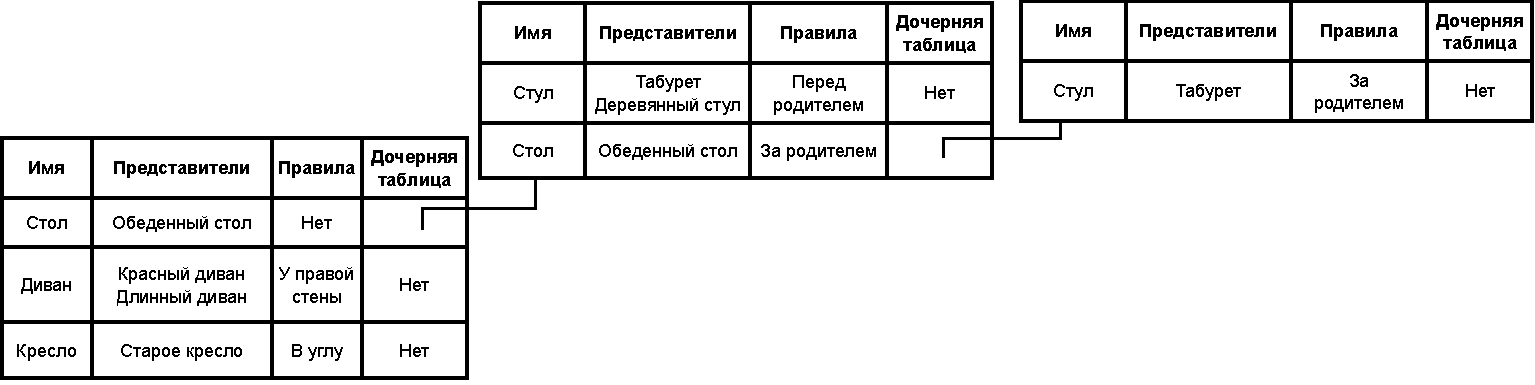
\includegraphics[width=\textwidth]{matmex-diploma-template-master/figures/data_table.pdf}
    \caption{Многоуровневая таблица объектов для размещения}
    \label{fig:data_table}
\end{figure}

\subsection{Алгоритм генерации интерьера}
Алгоритм генерации интерьера схож с рассмотренным в обзорной части, однако имеет ряд существенных отличий. Например, в целях уменьшения времени генерации объекты не могут быть удалены после размещения. Ниже приведено подробное описание искомого алгоритма. 

\begin{figure}
    \centering
    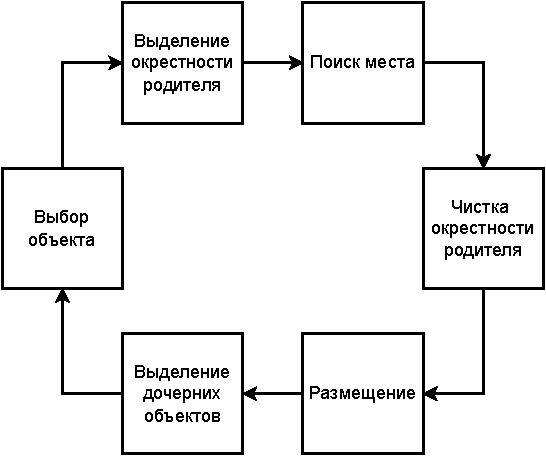
\includegraphics[width=0.4\textwidth]{matmex-diploma-template-master/figures/pcg.pdf}
    \caption{Последовательность шагов в алгоритме генерации интерьера}
    \label{fig:pcg}
\end{figure}

Шаги 1--6 повторяются, пока число объектов на сцене не достигло максимального или таблица объектов не пуста (рис. \ref{fig:pcg}).

\begin{enumerate}

    \item \textbf{Выбор объекта}. На данном этапе происходит выбор объекта для размещения с использованием генератора псевдослучайных чисел, который возвращает номер строки в таблице объектов и номер его представителя.

    \item \textbf{Выделение окрестности родителя}. Если выбранный предмет является дочерним, в зависимости от правил его размещения ячейки вокруг родительского объекта помечаются маркером \texttt{Oc\-cu\-pi\-ed\-For\-Chil\-dren}. На следующем шаге это позволит разместить дочерний объект рядом с родителем. 
    
    \item \textbf{Поиск места}. Поиск начинается с инициализации массива ячеек, соответствующих правилам размещения выбранного объекта. Например, если шкаф должен быть размещен у правой стены, то будут отобраны все незанятые клетки со статусом \texttt{Aga\-inst\-The\-Right\-Wall}. Из полученного массива случайным образом выбирается ячейка, которая должна стать центральной для объекта на сцене. В зависимости от наличия свободных ячеек вокруг объекта, на соответствие правилам  будет просмотрена и окрестность выбранной ячейки. Если окрестность не удовлетворяет правилам, искомая ячейка убирается из дальнейшего рассмотрения. Процесс будет повторятся, пока не будет найдена подходящая ячейка или массив не опустеет.  
    
    \item \textbf{Чистка окрестности родителя}. Если выбранный предмет является дочерним, то раннее помеченные \texttt{Oc\-cu\-pi\-ed\-For\-Chil\-dren} ячейки приобретают статус занятых. 
    
    \item \textbf{Размещение}. Если функция для поиска места вернула номер ячейки, то представитель объекта помещается в указанные координаты, а занятые ячейки (центральная и свободные ячейки указанные в правилах объекта) помечаются как \texttt{Occupied}. Иначе для выбранного представителя не существует свободного места и он убирается из рассмотрения, алгоритм возвращается к первому шагу. В случае, когда ни один представитель объекта не может разместиться --- из таблицы \enquote{удаляется} целая строка. Если окажется, что в первоначальной \texttt{DataTable} нет ни одной строки, процесс генерации останавливается.

    \item \textbf{Выделение дочерних объектов}. Если у размещенного объекта имеется таблица с дочерними объектами, алгоритм возвращается к первому шагу, принимая таблицу дочерних объектов за основную. Иначе возвращается к первому шагу с текущей \texttt{DataTable}. Когда таблица дочерних объектов становится пустой, алгоритм возвращается к случаю с родительской таблицей объектов. По этой причине на этапе смены таблиц информация о родителях и \texttt{CurrentDataTable} помещаются в стек.
    
\end{enumerate}

\begin{figure}
    \centering
    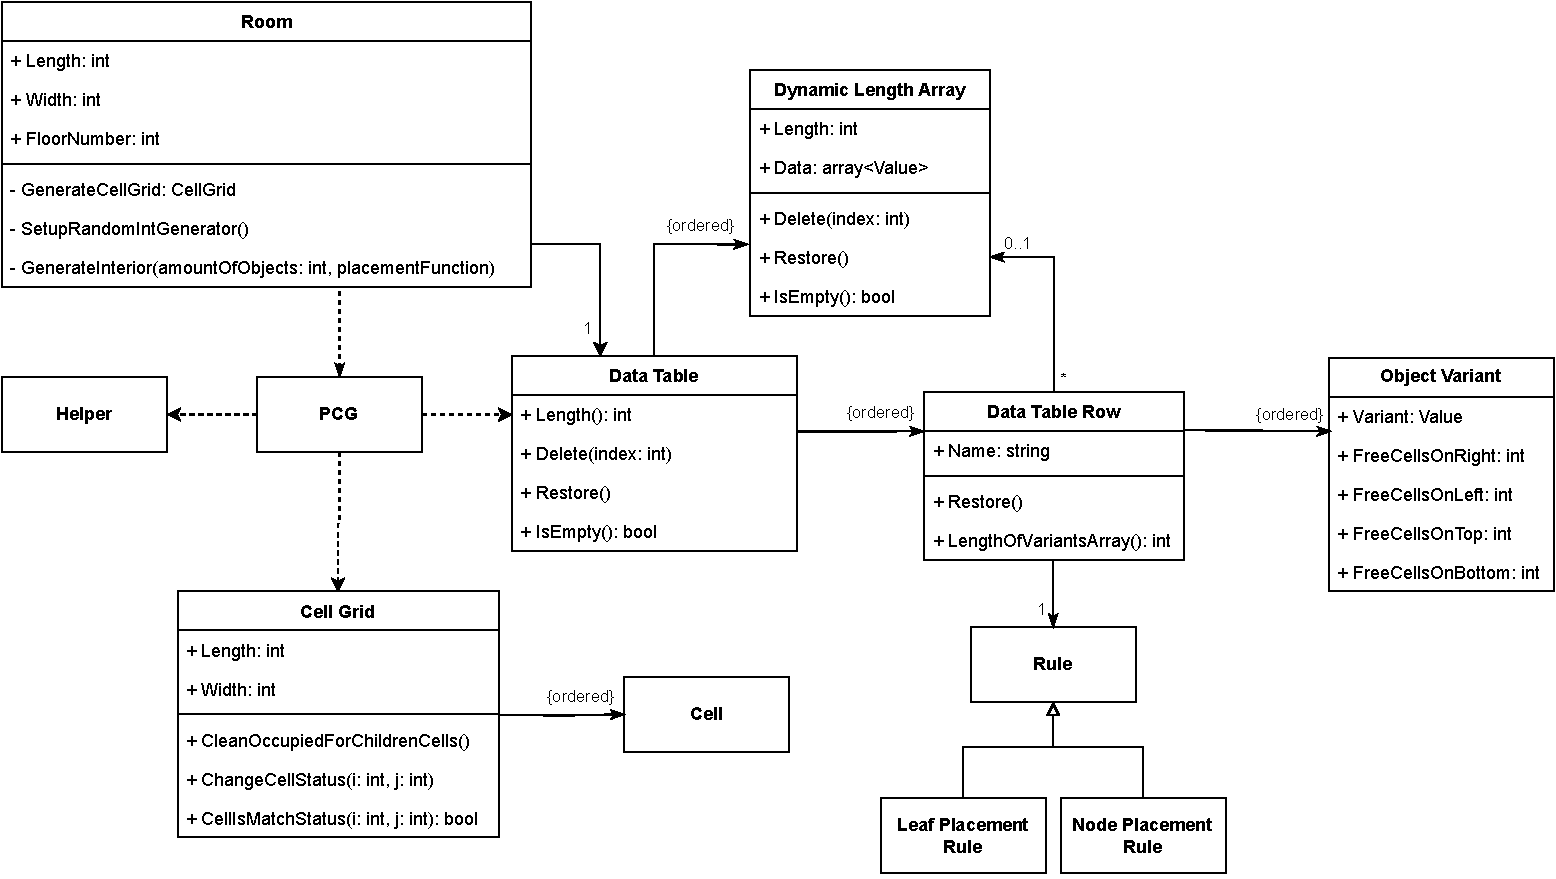
\includegraphics[width=\textwidth]{matmex-diploma-template-master/figures/uml.pdf}
    \caption{UML диаграмма классов библиотеки}
    \label{fig:uml}
\end{figure}

\subsection{Архитектура библиотеки}

Краткое описание модулей библиотеки представлено далее. Архитектура проекта представлена на UML диаграмме классов (диаг. \ref{fig:uml}). 

\begin{itemize}

    \item \textbf{Cell}. Данный модуль реализует ячейки, на которые разделяется комната, а также методы для проверки и изменения их состояний. Тип \texttt{Cell} представляет упомянутые раннее ячейки путем перечисления их состояний, например, \enquote{незанятая}, \enquote{угловая}, \enquote{зарезервированная для детей} и т.~д. В свою очередь, тип \texttt{CellGrid} инкапсулирует пространство для размещения в виде массива клеток. 
    
    \item \textbf{DataTable}. Модуль \texttt{DataTable} представляет инструменты для реализации входных данных алгоритма в виде таблиц, а также методы для удаления и восстановления ее строк. Типы, содержащиеся в модуле представлены далее.
        \begin{itemize}
            \item \texttt{LeafPlacementRule} и \texttt{NodePlacementRule} представляют возможные правила размещения для объектов. Тип \texttt{Rule} объединяет оба этих понятия.
    
            \item \texttt{ObjectVariant} описывает представителей объектов, дополненных размерами свободных ячеек вокруг них. Представитель может являться любым типом, совпадающим с сигнатурой функции размещения.
            
            \item \texttt{DataTableRow} представляет строку в таблице входных данных \texttt{DataTable}
        \end{itemize}
    
    \item \textbf{PCG} модуль содержит описанный алгоритм генерации.

    \begin{figure}
        \centering
        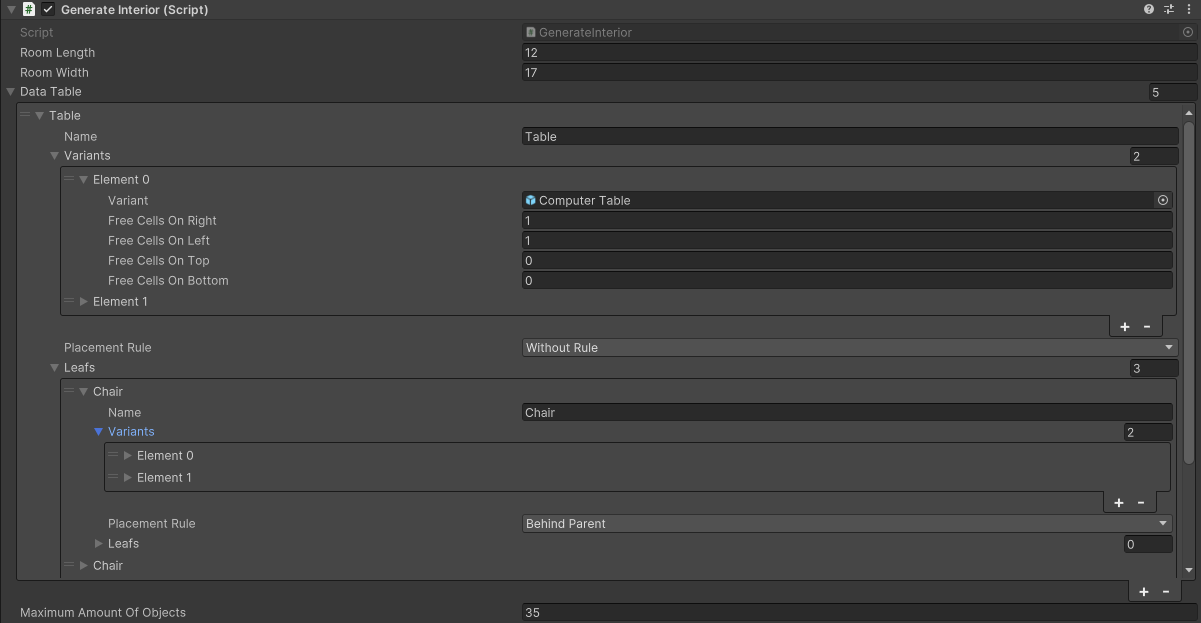
\includegraphics[width=\textwidth]{matmex-diploma-template-master/figures/inspector.png}
        \caption{Внешний вид панели Inspector в Unity}
        \label{fig:inspector}
    \end{figure}

    \item \textbf{Room} обобщает понятие комнаты. Модуль содержит информацию о ее размерах, номере этажа и таблице входных данных для декорирования. А также методы для разделения комнаты на ячейки, задания генератора псевдослучайных чисел и декорирования.
    
    \item \textbf{DynamicLengthArray} представляет массив переменной длины, используемый в представлении большинства структур библиотеки, в том числе \texttt{DataTable}. В отличие от честных динамических структур, изменение размера \texttt{DynamicLengthArray} не приводит к инициализации нового массива, а лишь сужает зону его видимости. Подобная механика, например, позволяет разным строкам \texttt{DataTable} ссылаться на одну дочернюю таблицу --- в конце итерации зона видимости вернется к прежнему значению и таблица \enquote{восстановится}. Другими словами, допустим, что объект \enquote{стол} породил все возможные дочерние объекты рядом. Как было описано раннее, при отсутствии свободного места, очередной листовой объект убирается из рассмотрения. Следовательно, дочерняя таблица окажется пустой, что станет проблемой для объекта \enquote{тумба}, ссылающегося на ту же дочернюю таблицу, что и \enquote{стол}. 
    
    \item \textbf{Helper} содержит вспомогательные функции.
    
\end{itemize}

Более подробно ознакомиться с API библиотеки можно на соответствующей странице GitHub Pages\footnote{https://polinasavelyeva.github.io/RoomInteriorGenerator/reference/index.html (дата обращения: \DTMdate{2024-01-2}).}.

Тестовое покрытие библиотеки составляет ~64\%. Такой процент был достигнут как с использованием ручных тестовых сценариев, так и при помощи тестирования на основе свойств.

\begin{figure}
    \centering
    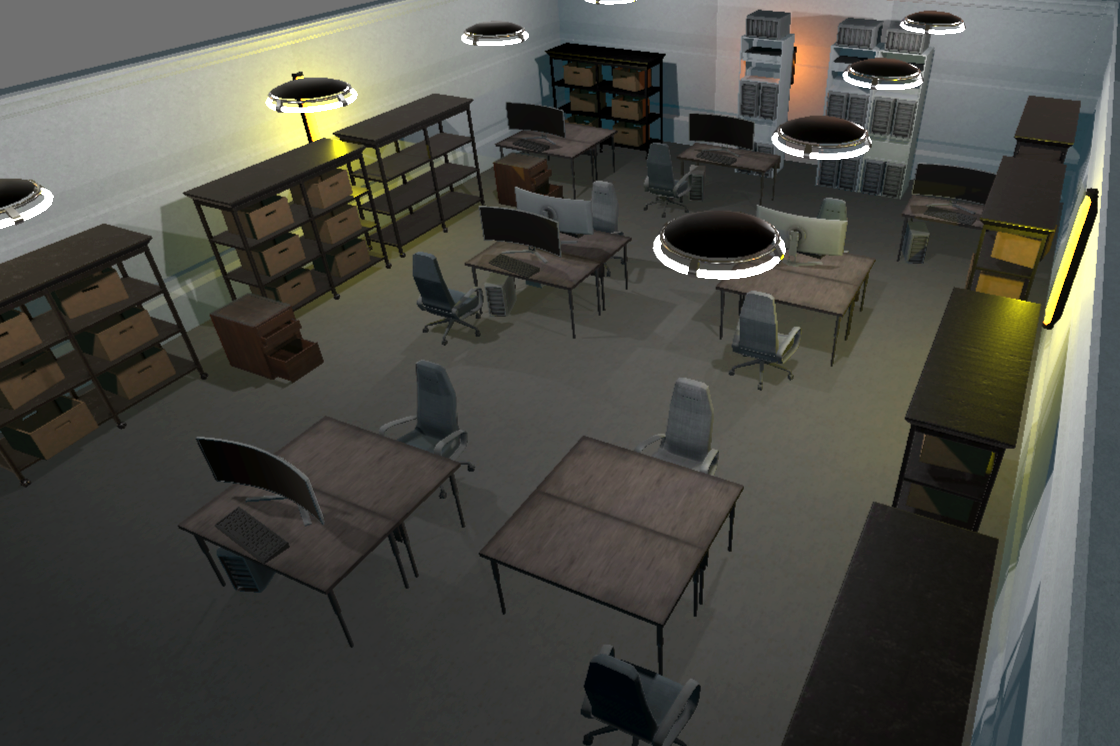
\includegraphics[width=0.45\textwidth]{matmex-diploma-template-master/figures/computing_center.png}
    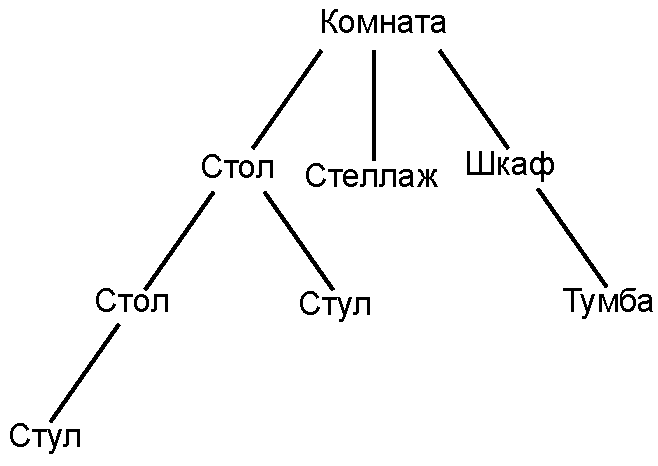
\includegraphics[width=0.45\textwidth]{matmex-diploma-template-master/figures/double_tables_tree.pdf}
    \caption{Процедурно заполненная комната с двойными столами (слева) и ее древовидное представление (справа)}
    \label{fig:double_table}
\end{figure}

\subsection{Реализация процедурной генерации в игре}

Логика генерации интерьера была реализована на панели Inspector (рис. \ref{fig:inspector}), содержащей свойства и компоненты объектов. Использование Inspector является распространенной практикой работы с Unity проектами, которая облегчает взаимодействие с игровыми скриптами и создает четкое разделение на программную и дизайнерскую составляющие. 

Каждое помещение заранее разделяется на зоны, необходимые к декорированию, такой прием позволяет, например, разместить предметы над и под складской лестницей. В левом верхнем углу каждой зоны размещается пустой игровой объект (которому \enquote{присваивают} скрипт генерации), являющийся началом координат для всех порожденных предметов мебели. Для получения ожидаемого результата следует дополнительно проверить, сходятся ли локальная координатная система области для декорирования и глобальная у игрового мира. 

Стоит обратить внимание и на то, в каком месте находится центр размещаемых объектов и на какой угол они изначально отклонены по каждой из осей. Некоторые объекты намеренно не соответствуют этим правилам, например, дочерний объект может быть заранее повернут на определенный угол --- такой прием позволил воссоздать сложную иерархическую структуру с двойными столами, представленную на рис. \ref{fig:double_table}. Примеры полученных комнат приведены на рис. \ref{fig:tech_warehouse}, \ref{fig:laboratory}.

\begin{figure}
    \centering
    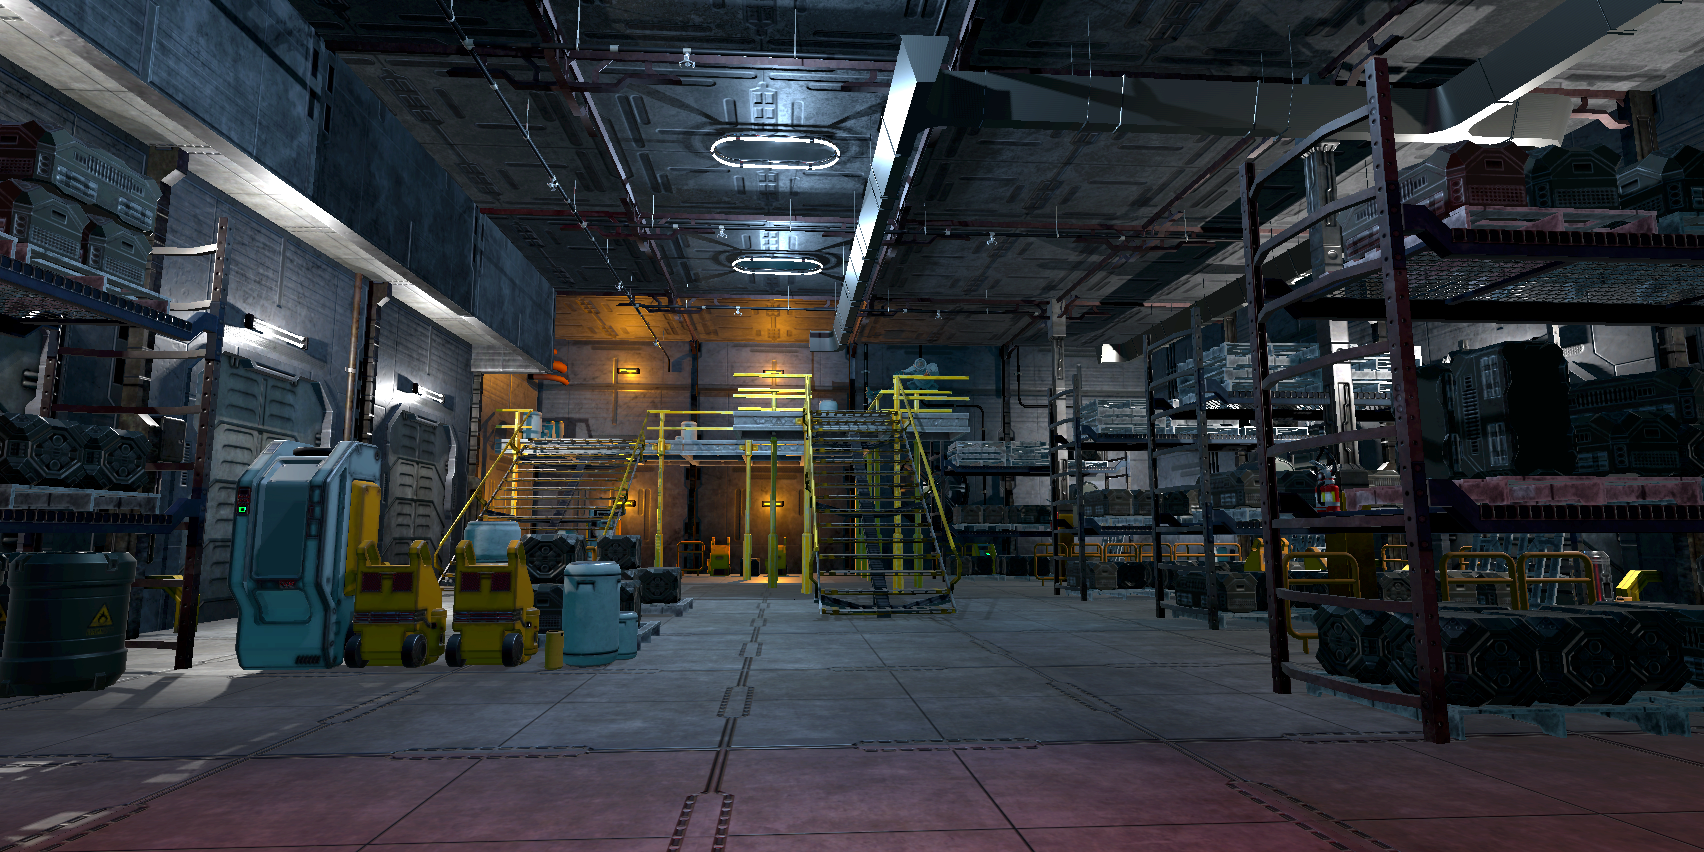
\includegraphics[width=\textwidth]{matmex-diploma-template-master/figures/tech_warehouse.png}
    \caption{Процедурно заполненное складское помещение}
    \label{fig:tech_warehouse}
    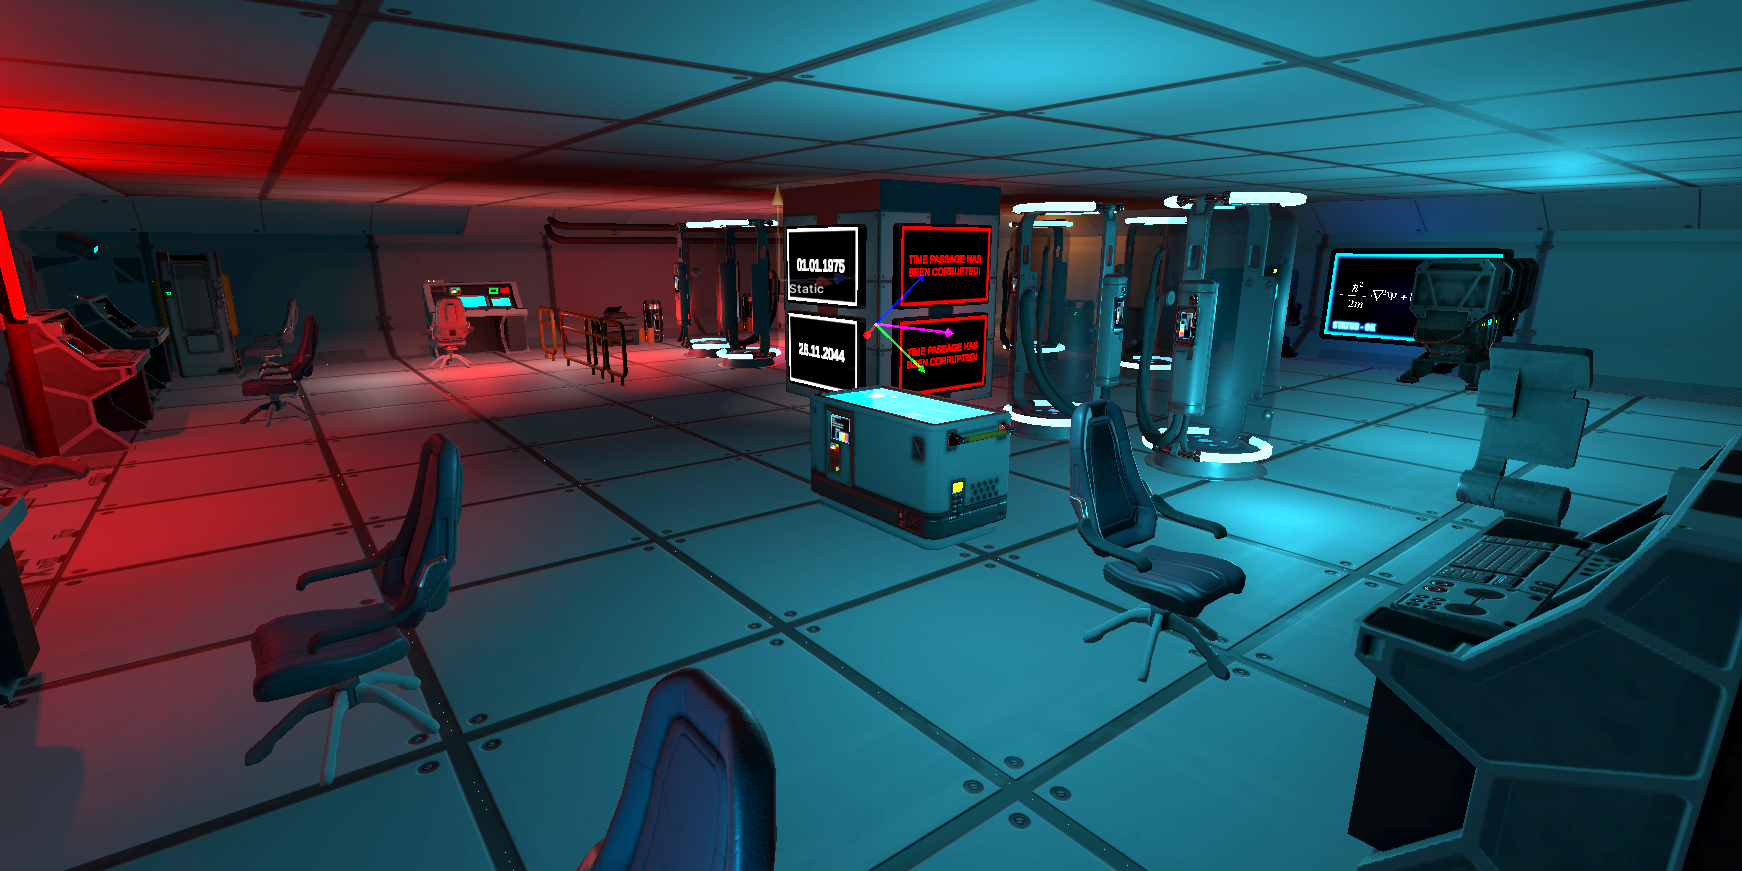
\includegraphics[width=\textwidth]{matmex-diploma-template-master/figures/laboratory.png}
    \caption{Процедурно заполненное лабораторное помещение}
    \label{fig:laboratory}
\end{figure}